

\section{Les lois a posteriori}
La loi a posteriori est utilis\'ee pour estimer une vari\'et\'e des param\`etres de mod\`ele d'int\'erêt , tels que la moyenne, la m\'ediane, le mode, et ainsi de suite. \par Il est possible de construire des \textbf{intervalles / r\'egions cr\'edibles} directement \`a partir de la distribution a posteriori (contrairement \`a "la confiance" intervalles d'inf\'erence fr\'equentiste).
\newl \'etant donn\'e une loi a posteriori sur un param\`etre $\theta$, un $1-\alpha$ intervalle cr\'edible $[L,U]$  est l'intervalle tel que 
$$ P(L \leq \theta \leq U\mid D)\geq 1-\alpha.$$
Parce que la distribution a posteriori est une loi compl\`ete sur les param\`etres, il est possible de faire toutes sortes de d\'eclarations probabilistes sur leurs valeurs, telles que:
\begin{itemize}[noitemsep]
	\item ``Je suis 95\% sûr que la vraie valeur du param\`etre est plus grande que 0.5.''
	\item Il y a 50\% de chances que $\theta_1$ soit plus grand que $\theta_2$.
  \item etc.
\end{itemize}
La meilleure approche consiste \`a construire l'intervalle cr\'edible des valeurs $\theta$ en utilisant \textbf{l'intervalle HPD}
(HPD pour Highest Posterior
Density, soit densit\'e a posteriori la plus forte), c'est-\`a-dire \`a d\'efinir une r\'egion $C_k$ dans l'espace des param\`etres avec
$$ C_k = \left\{\theta: P(\theta\mid D)\geq k\right\},$$
où $k$ est le plus grand nombre tel que
$$ \int_{C_k} P(\theta\mid D)\, d\theta = 1-\alpha.$$
L'effet est ordinairement de trouver la plus petite r\'egion $C_k$ (en mesure) \`a satisfaire au crit\`ere. \par La valeur $k$ peut être consid\'er\'ee comme la hauteur d'une ligne horizontale (ou hyperplan, dans le cas des a posteriori multivari\'ees) superpos\'ee sur la distribution a posteriori et dont l'intersection(s) avec cette derni\`ere d\'efinit une r\'egion sur laquelle l'int\'egrale de la distribution a posteriori est $1-\alpha$. Dans la plupart des cas, la valeur k peut être trouv\'ee num\'eriquement. 
\begin{Exemple}
\textit{HPDs, \'elections et collecte it\'erative de donn\'ees.} C'est une ann\'ee d'\'election et vous voulez savoir si la population en g\'en\'eral pr\'ef\`ere le candidat $A$ ou le candidat $B$. Un sondage r\'ecemment publi\'e indique que parmi $400$ personnes \'echantillonn\'ees au hasard, $232$ ont pr\'ef\'er\'e le candidat $A$, tandis que les autres ont pr\'ef\'er\'e le candidat $B$.
\begin{enumerate}[noitemsep,label=(\alph*)]
\item Supposons qu'avant la publication du sondage, vous pensiez que la pr\'ef\'erence g\'en\'erale suit une loi uniforme. Quel est l'HPD de $95\%$ sur votre croyance apr\`es avoir appris le r\'esultat du sondage?  
\newl 
\textbf{Solution}: notons la pr\'ef\'erence pour le candidat $A$ par 1, et la pr\'ef\'erence pour le candidat $B$ par 0.  On peut utiliser la fonction R  \texttt{BernBeta()} comme dans l'Exemple~\ref{ex4}. \`a l'invite de commande R, tapez
\newl \footnotesize \texttt{> post=BernBeta(c(1,1),c(rep(1,232),rep(0,168))) }\normalsize\newl
 donnant une a post\'eriori avec un  95\% HPD de $0.531$ \`a $0.628$ pour la probabilit\'e du candidat $A$.
\begin{center}		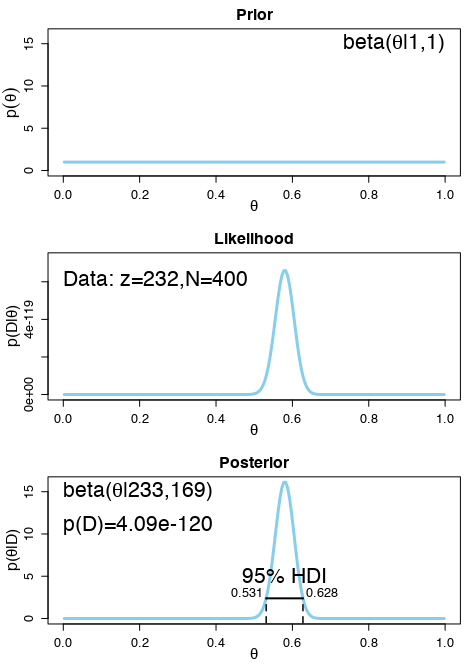
\includegraphics[width=\linewidth]{Images/example8a.png}
\end{center}
\item  D'apr\`es le sondage, est-il cr\'edible de croire que la population est \'egalement divis\'ee dans ses pr\'ef\'erences entre des candidats? \newl \textbf{Solution:} l'intervalle HPD de la Partie (a) montre que $\theta=0.5$ ne fait pas partie des valeurs cr\'edibles, il n'est donc pas cr\'edible de croire que la population est \'egalement divis\'ee dans ses pr\'ef\'erences (au niveau de 95\%).
\item Vous souhaitez effectuer un sondage compl\'ementaire pour affiner votre estimation de la pr\'ef\'erence de la population. Dans le sondage compl\'ementaire, vous \'echantillonnez au hasard $100$ personnes et vous constatez que $57$ d'entre elles pr\'ef\`erent le candidat $A$. En supposant que l'opinion des gens n'a pas chang\'e entre les sondages, quel est l'intervalle HPD de 95\% sur la distribution a posteriori? \newl \textbf{Solution:} 
\`a l'invite de commande R, tapez \newl \footnotesize \texttt{
> post=BernBeta(post,c(rep(1,57),rep(0,43)))}\normalsize \newl
donne la figure ci-dessous. Le 95\% intervalle HPD est a un peu plus \'etroit pour la pr\'ef\'erence du candidat $A$, de 0.534 \`a 0.621.
\begin{center}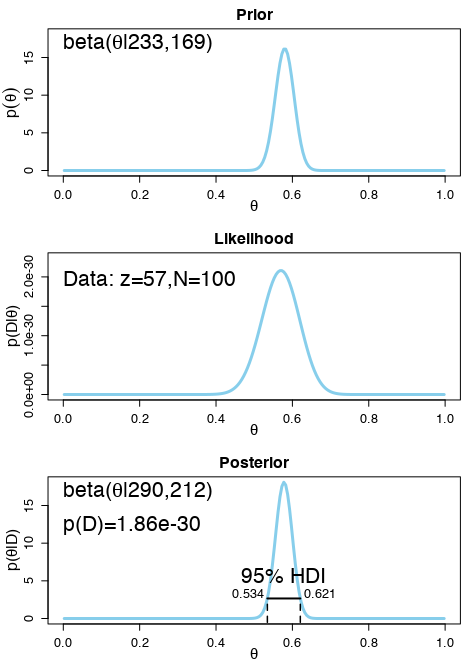
\includegraphics[width=\linewidth]{Images/example8b.png}\end{center}
 \item Sur la base du sondage compl\'ementaire, est-il cr\'edible de croire que la population est \'egalement divis\'ee dans ses pr\'ef\'erences entre les candidats? \newl\textbf{Solution:} L'intervalle HPD de la partie $(c)$ exclut $\theta=0.5$; le sondage compl\'ementaire et le sondage initial sugg\`erent que la population n'est pas divis\'ee \'egalement (et pr\'ef\`ere en fait le candidat $A$).
\end{enumerate}
\end{Exemple}

\subsection{Les m\'ethodes de Monte-Carlo par Cha\^{\i}ne de Markov (MCMC)}
La v\'eritable puissance de l'inf\'erence bay\'esienne se fait surtout sentir lorsque les sp\'ecifications du mod\`ele conduisent \`a un a posteriori qui ne peut être manipul\'e analytiquement; dans ce cas, il est habituellement possible de recr\'eer un ensemble synth\'etique (ou simul\'e) de valeurs qui partagent les propri\'et\'es d'un a posteriori donn\'e. Ces processus sont connus sous le nom des \textbf{simulations de Monte Carlo}.  Une \textbf{Cha\^{\i}ne de Markov} est un ensemble ordonn\'e et index\'e de variables al\'eatoires (un processus stochastique) dans lequel les valeurs des quantit\'es \`a un \'etat donn\'e ne d\'ependent, de façon probabiliste, que des valeurs des quantit\'es \`a l'\'etat pr\'ec\'edent.  Les m\'ethodes de \textbf{Monte-Carlo par Cha\^{\i}ne de Markov} (MCMC) sont une classe d'algorithmes pour l'\'echantillonnage \`a partir d'une loi de probabilit\'e bas\'ee sur la construction d'une cha\^{\i}ne de Markov avec la loi d\'esir\'ee comme loi d'\'equilibre. L'\'etat de la cha\^{\i}ne apr\`es un certain nombre d'\'etapes est alors utilis\'e comme \'echantillon de la loi souhait\'ee. La qualit\'e de l'\'echantillon s'am\'eliore en fonction du nombre d'\'etapes. \newl Les techniques MCMC sont souvent appliqu\'ees pour r\'esoudre des probl\`emes d'int\'egration et d'optimisation dans des espaces de grandes dimensions. Ces deux types de probl\`emes jouent un rôle fondamental dans l'apprentissage machine (en anglais machine learning)la physique, les statistiques, l'\'econom\'etrie et l'analyse des d\'ecisions. Par exemple, compte tenu des variables $\theta\in\Theta$ et des donn\'ees data $D$, les probl\`emes d'int\'egration suivants (g\'en\'eralement insolubles) sont principales \`a l'inf\'erence bay\'esienne:
\begin{itemize}
	\item \textbf{La normalisation} - pour obtenir la distribution a posteriori $P(\theta \mid  D)$ \'etant donn\'ee la distribution a priori $P(\theta)$ et la vraisemblance $P(D\mid \theta)$, le facteur de normalisation (d\'enominateur) du th\'eor\`eme de Bayes doit être calcul\'e
	$$P(\theta \mid  D) = \frac{p(\theta)  P(D\mid \theta)}{\int P(D\mid \theta) P(\theta) d\theta}. $$

  \item \textbf{La marginalisation} - \'etant donn\'ee la distribution a posteriori conjointe de $(\theta,x)$, on est souvent int\'eress\'es par la distribution a posteriori marginale
	$$ P(\theta\mid D) = \int P(\theta,x\mid D) dx.$$
	
	\item \textbf{l'esp\'erance}- l'objectif final de l'analyse est souvent pour obtenir des statistiques sommaires de la forme 
	       $$ E(f(\theta)) = \int_{\Theta} f(\theta) P(\theta\mid D) d\theta $$
				pour une fonction d'int\'erêt (c-\`a-d $f(\theta) =\theta$ (la moyenne), ou $f(\theta) = (\theta-E(\theta))^{2}$ (la variance)). 
\end{itemize}

\subsubsection*{L'algorithme de Metropolis-Hastings (MH)}
L'algorithme de Metropolis-Hastings (MH) est un type sp\'ecifique de processus de Monte Carlo; il fait probablement partie des dix algorithmes qui ont r\'ecemment eu la plus grande influence sur le developpement et la pratique de la science et de l'ing\'enierie. \par MH g\'en\`ere une marche al\'eatoire (c'est-\`a-dire qu'elle g\'en\`ere une succession d'\'echantillons a posteriori) de façon \`a ce que chaque \'etape de la marche soit \textbf{compl\`etement ind\'ependante} des \'etapes pr\'ec\'edentes; la d\'ecision de rejeter ou d'accepter l'\'etape propos\'ee est \'egalement ind\'ependante de l'histoire de la marche. \newl Tout processus pour lequel l'\'etape actuelle est ind\'ependante (oubli\'ee) des \'etats pr\'ec\'edents, \`a savoir
$$P(X_{n+1}=x\mid X_1=x_1,\ldots,X_n=x_n)=P(X_{n+1}=x\mid X_n=x_n)$$ pour tout $n$, $X_j$ et $x_j$, $j=1,\ldots, n$, est appel\'e un \textbf{processus de Markov (du premier ordre)}, et une succession de ces \'etapes est une cha\^{\i}ne de Markov(du premier ordre). \newl MH utilise une loi candidate ou de proposition pour la distribution a posteriori, disons q($\cdot$, $\theta$), où $\theta$ est un vecteur de param\`etres qui est fix\'e par les param\`etres de r\'eglage de l'appel utilisateur; MH construit ensuite une cha\^{\i}ne de Markov en proposant une valeur pour $\theta$ \`a partir de cette loi candidate, puis en acceptant ou en rejetant cette valeur (avec une certaine probabilit\'e). \newl Th\'eoriquement, la loi de proposition peut être presque n'importe quelle loi, mais en pratique il est recommand\'e de choisir des lois (vraiment) simples: une normale si le param\`etre d'int\'erêt peut être n'importe quel nombre r\'eel (par exemple $\mu$), ou une log-normale si elle a un support positif (disons $\sigma^{2}$). \newl
L'algorithme de \textbf{Metropolis-Hastings}(MH) simule des \'echantillons \`a partir d'une loi de probabilit\'e en utilisant la fonction de densit\'e conjointe compl\`ete et des lois de proposition (ind\'ependantes) pour chacune des variables d'int\'erêt.  L’algorithme MH passe au travers des \'etapes suivantes \`a chaque it\'eration en recommençant ces \'etapes pour $i$ allant de 0 \`a $N$.
\begin{algorithm}
\SetAlgoLined
\caption{L'algorithme de Metropolis-Hastings}
\text{G\'en\'erer: } $x^{(0)}\sim q(x)$ \\

\it{Propose: } $x^* \sim q(x^{(i)}\mid  x^{(i-1)})$ \\
\it{Calculer la probabilit\'e d'acceptation: } 
$$ \alpha(x^*\mid x^{(i-1)}) = min\left\{1, \frac{q(x^{(i-1)}\mid x^*)\pi(x^*)}{q(x^*\mid x^{(i-1)})\pi(x^{(i-1)})}\right\}$$ \\
\text{Prendre: }
\[
   x^{(i)} = 
    \begin{cases}
        x^* & \text{avec probabilit\'e $\alpha$} \\
        x^{(i-1)} & \text{avec probabilit\'e $1-\alpha$} \\
    \end{cases}
\]
\label{algorithmMH}
\end{algorithm}
\par \noindent La premi\`ere \'etape consiste \`a initialiser la valeur de l'\'echantillon pour chaque variable al\'eatoire (souvent obtenue par \'echantillonnage \`a partir de la loi a priori de la variable). La boucle principale de l'Algorithme 1 comprend trois composantes: 
\begin{itemize}[noitemsep]
	\item \textbf{g\'en\'erer un \'echantillon de candidats} $x^{*}$ \`a partir de la loi de proposition  $q(x^{(i)}\mid  x^{(i-1)})$;
	\item \textbf{calculer la probabilit\'e d'acceptation} via la fonction d'acceptation $\alpha(x^{*}\mid x^{(i-1)})$ sur la base de la loi de proposition et de la densit\'e conjointe compl\`ete  $\pi(\cdot)$;
	\item \textbf{accepter l'\'echantillon candidat} avec la probabilit\'e $\alpha$,la probabilit\'e d'acceptation, sinon le \textbf{rejeter}. 
\end{itemize}

\begin{Exemple} \textbf{L'algorithme MH et la r\'egression lin\'eaire simple}. Les \textbf{donn\'ees d'essai} pour cet exemple sont g\'en\'er\'ees \`a l'aide du code suivant.
\begin{lstlisting}
t.A <- 10 # la vrai valeur de la pente 
t.B <- 0 # la vrai valeur de l'ordonn\'ee \`a l'origine
t.sd <- 20 # La vrai valeur de la variance de l'erreur al\'eatoire 
s.Size <- 50 # la taille de l'\'echantillon
# cr\'eer des valeur ind\'ependantes de x
x <- (-(s.Size-1)/2):((s.Size-1)/2)
# cr\'eer des valeur d\'ependantes  selon l'\'equation  ax + b + N(0,sd)
y <-  t.A * x + t.B + rnorm(n=s.Size,mean=0,sd=t.sd)
plot(x,y, main="Donn\'ees d'essai")
\end{lstlisting}
\noindent Remarquez que les valeurs $x$ sont \'equilibr\'ees autour de z\'ero pour "d\'ecorr\'eler" la pente et l'ordonn\'ee \`a l’origine. Le r\'esultat devrait ressembler \`a la graphique ci-dessous. 
\begin{center}
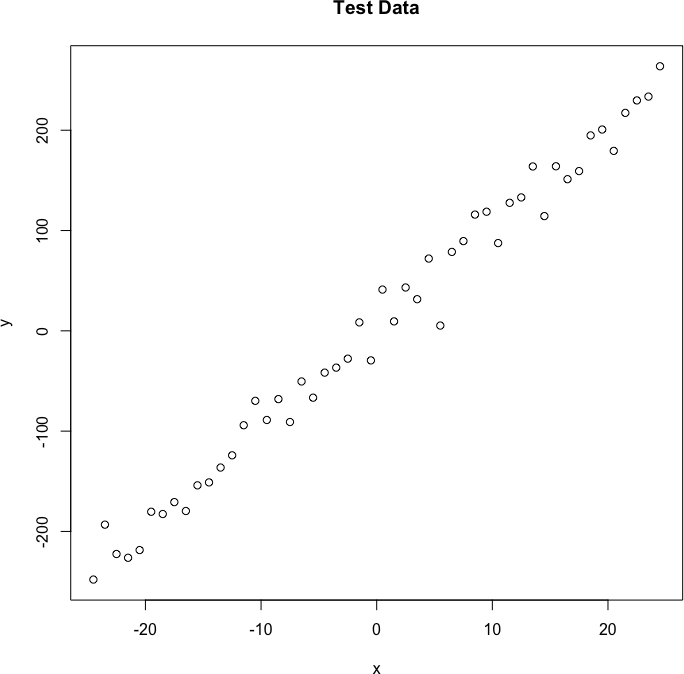
\includegraphics[width=0.95\linewidth]{Images/example9a.png}
\end{center}
\item \textbf{D\'efinition du mod\`ele statistique.} L'\'etape suivante consiste \`a sp\'ecifier le mod\`ele statistique. Nous savons d\'ej\`a que les donn\'ees \'etaient cr\'e\'ees avec une relation lin\'eaire $y = ax + b$ ainsi qu'un mod\`ele d'erreur normal  $N(0,sd)$ avec l'\'ecart-type $sd$, donc nous pourrions aussi bien utiliser le même mod\`ele pour l'ajustement et voir si nous pouvons r\'ecup\'erer nos valeurs de param\`etres originales. Notez cependant qu'en g\'en\'eral, le mod\`ele de g\'en\'eration est inconnu. \\
\textbf{D\'erivation de la fonction de vraisemblance \`a partir du mod\`ele}. Un mod\`ele lin\'eaire de la forme $y = ax + b + N(0,sd)$ prend la param\`etres $(a, b, sd)$ comme entr\'ees. Le r\'esultat devrait être la probabilit\'e d'obtenir les donn\'ees de test dans le cadre de ce mod\`ele: dans ce cas, il suffit de calculer la diff\'erence entre les pr\'edictions $y = ax + b$ t le y observ\'e, puis de rechercher la probabilit\'e (\`a l'aide de la fonction \textit{dnorm}) que de tels \'ecarts se produisent.
\begin{lstlisting}
likehd <- function(param){
    a = param[1]
    b = param[2]
    sd = param[3]
    pred = a*x + b
    singlelikelihoods = dnorm(y, mean = pred, sd = sd, log = T)
    sumll = sum(singlelikelihoods)
    return(sumll) }
# Exemple: Faire la graphe du profil de la vraisemblance  de la pente a
s.values <- function(x){return(likehd(c(x, t.B, t.sd)))}
s.likehds <- lapply(seq(1/2*t.A, 3/2*t.A, by=.05), s.values)
plot(seq(1/2*t.A, 3/2*t.A, by=.05), s.likehds , type="l", xlab = "Les valeurs du parametre de pente a", ylab = "Log de la vraisemblance")
\end{lstlisting}
Pour illustrer, les derni\`eres lignes du code tracent la Vraisemblance pour une gamme de valeurs param\'etriques du param\`etre de pente $a$. Le r\'esultat devrait ressembler au graphe ci-dessous. 
\begin{center}
		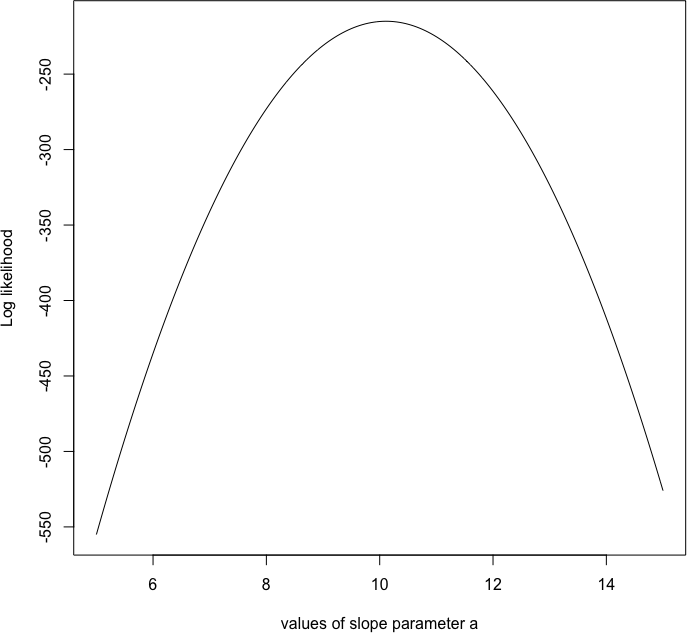
\includegraphics[width=0.95\linewidth]{Images/example9b.png}
\end{center}
\item \textbf{D\'efinir les a priori.} Dans l'analyse bay\'esienne, l'\'etape
suivante est toujours n\'ecessaire: nous devons sp\'ecifier une loi a priori pour chacun des param\`etres du mod\`ele. Pour simplifier les choses, nous utiliserons une loi uniforme pour les trois param\`etres et nous utiliserons des lois normales pour chacun d'entre eux.\footnote{Nous travaillons avec les logarithmes de toutes quantit\'es, de sorte que la vraisemblance est une somme et non un produit comme ce serait habituellement le cas.} 
\begin{lstlisting}
# Prior distribution
prior <- function(param){
    a = param[1]
    b = param[2]
    sd = param[3]
    aprior = dunif(a, min=0, max=2*t.A, log = T)
    bprior = dnorm(b, mean=t.B, sd = 5, log = T)
    sdprior = dunif(sd, min=0, max=2*t.sd, log = T)
    return(aprior+bprior+sdprior)
}
\end{lstlisting}

\item \textbf{L'a posteriori.} Le produit de la distribution a priori par la vraisemblance est la quantit\'e r\'eelle avec laquelle MCMC travaille (il n'est pas, strictement parlant, la distribution a posteriori car il n'est pas normalis\'e).

\begin{lstlisting}
posterior <- function(param){
   return (likehd(param) + prior(param))
}
\end{lstlisting}
 \item \textbf{Appliquer l'algorithme MH.} L'une des applications les plus fr\'equentes de le MH (comme dans cet exemple) est l'\'echantillonnage par la densit\'e a posteriori en statistiques bay\'esienne.\footnote{L'algorithme peut être utilis\'e pour \'echantillonner \`a partir de n'importe quelle fonction int\'egrable.} L'objectif de l'algorithme est de sauter dans l'espace des param\`etres, mais de mani\`ere \`a avoir la probabilit\'e d'atterrir en un point soit proportionnel \`a la fonction dont nous \'echantillonnons (c'est ce que l'on appelle g\'en\'eralement la fonction cible). Dans ce cas, la fonction cible est la fonction a posteriori d\'efinie pr\'ec\'edemment. \newl Pour ce faire, il faut 
\begin{enumerate}[noitemsep]
\item commencer par un vecteur de param\`etre al\'eatoire;
\item choisir un nouveau vecteur de param\`etre proche de l'ancienne valeur sur la base d'une certaine densit\'e de probabilit\'e (la fonction de proposition), et 
\item sauter \`a ce nouveau point avec une probabilit\'e $\alpha=\min\{1,g(\text{new})/g(\text{old})\}$, où $g$ est la fonction cible.\end{enumerate}
La loi des vecteurs de param\`etres (MH visites) converge vers la loi cible  $g$.
\begin{lstlisting}
######## MH ################
proposalfunction <- function(param){
    return(rnorm(3,mean = param, sd= c(0.1,0.5,0.3)))
}
 
run_metropolis_MCMC <- function(startvalue, iterations){
    chain = array(dim = c(iterations+1,3))
    chain[1,] = startvalue
    for (i in 1:iterations){
        proposal = proposalfunction(chain[i,])
         
        probab = exp(posterior(proposal) - posterior(chain[i,]))
        if (runif(1) < probab){
            chain[i+1,] = proposal
        }else{
            chain[i+1,] = chain[i,]
        }
    }
    return(chain)
}
 
startvalue = c(4,0,10)
chain = run_metropolis_MCMC(startvalue, 10000)
burnIn = 5000
acceptance = 1-mean(duplicated(chain[-(1:burnIn),]))
\end{lstlisting}
Les premi\`eres \'etapes de l'algorithme peuvent être biais\'ees par le processus d'initialisation; ils sont g\'en\'eralement rejet\'es pour l'analyse (c'est ce qu'on appelle \textbf{le temps de rodage}).  
\newl Un r\'esultat int\'eressant \`a \'etudier est le taux d'acceptation: combien de fois une proposition a-t- elle \'et\'e rejet\'ee par le crit\`ere d'acceptation du MH? Le taux d'acceptation peut être influenc\'e par la fonction de proposition: en g\'en\'eral, plus la fonction propos\'ee est proche de la derni\`ere plus le taux d'acceptation est \'elev\'e.  Les taux d'acceptation tr\`es \'elev\'es, cependant, ne sont habituellement pas b\'en\'efiques, car cela implique que l'algorithme «reste» dans le même voisinage ou point, ce qui se traduit par un sondage sous-optimal de l'espace des param\`etres (il y a un \textbf{m\'elange} tr\`es faible). Des taux d'acceptation compris entre $20\%$ et $30\%$ sont consid\'er\'es comme optimaux pour des applications typiques \cite{BDA_N11}.\newl
Enfin, nous pouvons tracer les r\'esultats. 
\begin{lstlisting}
### Summary: #######################
 par(mfrow = c(2,3))
hist(chain[-(1:burnIn),1],nclass=30, , main="la distribution a posteriori de a", xlab="La vrais valeur = La ligne rouge")
abline(v = mean(chain[-(1:burnIn),1]))
abline(v = t.A, col="red")
hist(chain[-(1:burnIn),2],nclass=30, main="la distribution a posteriori de b", xlab="La vrais valeur = La ligne rouge")
abline(v = mean(chain[-(1:burnIn),2]))
abline(v = t.B, col="red")
hist(chain[-(1:burnIn),3],nclass=30, main="la distribution a posteriori de sd", xlab="La vrais valeur = La ligne rouge")
abline(v = mean(chain[-(1:burnIn),3]))
abline(v = t.sd, col="red")
plot(chain[-(1:burnIn),1], type = "l", xlab="La vrais valeur = La ligne rouge" , main = "Les valeurs de cha\^{\i}ne de a",)
abline(h = t.A, col="red")
plot(chain[-(1:burnIn),2], type = "l", xlab="La vrais valeur = La ligne rouge" , main = "Les valeurs de cha\^{\i}ne de b",)
abline(h = t.B, col="red")
plot(chain[-(1:burnIn),3], type = "l", xlab="La vrais valeur = La ligne rouge" , main = "Les valeurs de cha\^{\i}ne de sd",)
abline(h = t.sd, col="red")
# for comparison:
summary(lm(y~x))
\end{lstlisting}
\begin{center}
		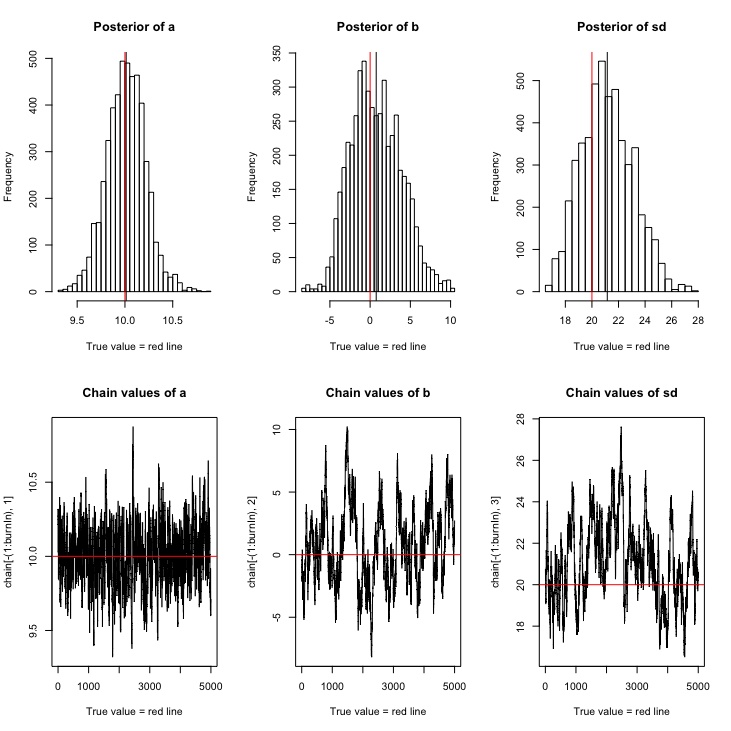
\includegraphics[width=1.0\linewidth]{Images/example9c.png}
\end{center}
Les graphes r\'esultants devraient ressembler \`a celles qui ont \'et\'e vues dans la colonne de droite: la ligne sup\'erieure indique les estimations $a$ posteriori pour la pente $a$, l'ordonn\'ee \`a l’origine $b$ et l'\'ecart type de l'erreur $sd$;la ligne inf\'erieure montre la cha\^{\i}ne de Markov des valeurs des param\`etres.  Nous r\'ecup\'erons (plus ou moins) les param\`etres d'origine qui ont \'et\'e utilis\'es pour cr\'eer les donn\'ees, et il y a une certaine zone autour des valeurs a posteriori les plus \'elev\'ees qui montre \'egalement un certain appui par les donn\'ees, qui est l'\'equivalent bay\'esien des intervalles de confiance.\\
Les lois a posteriori ci-dessus sont des lois \textbf{marginales}, les lois conjoints sont indiqu\'ees ci- dessous. 
\begin{center}
		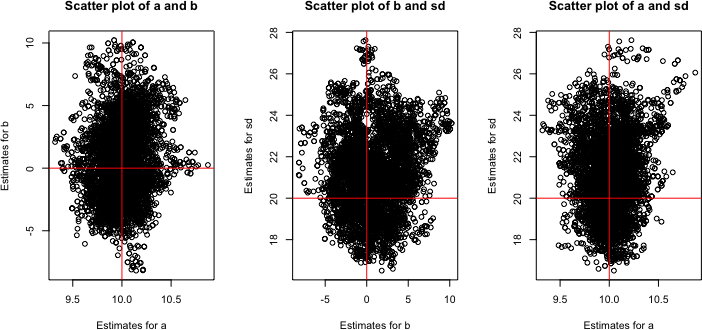
\includegraphics[width=0.99\linewidth]{Images/example9d.png}
\end{center}
\`a titre de comparaison, la fonction \texttt{lm()} dans R donne les estimations suivantes: $a: 9.9880$ (se: 0.2092), $b: 0.5840$ (se: 3.0185), and $sd = 21.34$ (48 d.f.).
\end{Exemple}

\subsection*{Exercices}
\begin{Exercice} Un groupe d'adultes fait une exp\'erience simple d'apprentissage:lorsqu'ils voient les deux mots \textit{radio} et \textit{oc\'ean}  apparaissent simultan\'ement sur un \'ecran d'ordinateur, on leur demande d'appuyer sur la touche F du clavier; chaque fois que les mots \textit{radio} et \textit{montagne} apparaissent \`a l'\'ecran, on leur demande d'appuyer sur la touche J.  Apr\`es plusieurs r\'ep\'etitions d'exercices, deux nouvelles tâches sont introduites: dans la premi\`ere, le mot \textit{radio} appara\^{\i}t tout seul et les participants sont invit\'es \`a donner la meilleure r\'eponse (F ou J) en fonction de ce qu'ils ont appris auparavant; dans la seconde, les mots \textit{oc\'ean} et \textit{montagne} apparaissent simultan\'ement et les participants sont \`a nouveau invit\'es \`a donner la meilleure r\'eponse. Ceci est r\'ep\'et\'e avec 50 personnes. Les donn\'ees montrent que, pour le premier test, 40 participants ont r\'epondu par F et 10 par J; tandis que pour le deuxi\`eme test, 15 ont r\'epondu par F et 35 par J. Les gens sont-ils biais\'es vers F ou vers J pour l'un des deux tests? Pour r\'epondre \`a cette question, supposez une a priori uniforme et utilisez un intervalle HPD de $95\%$ pour d\'ecider quels biais peuvent être d\'eclar\'es cr\'edibles.
\label{ex4.2.1} 
\end{Exercice}

%----------------------------------------------------------------------------------------
%----------------Uncertainty-------------------------------------------------------------
%----------------------------------------------------------------------------------------

\section{L'incertitude}
Selon \cite{BDA_GCSDVR}, \begin{quote}la caract\'eristique principale de l'inf\'erence bay\'esienne est la quantification directe de l'incertitude.\end{quote}
L'approche bay\'esienne Pour mod\'eliser l'incertitude particuli\`erement utile lorsque:
\begin{itemize}[noitemsep]
	\item les donn\'ees disponibles sont limit\'ees;
	\item il y a une certaine inqui\'etude concernant le sur- ajustement(``overfitting,'' en anglais);
	\item certains faits ont plus de chances d'être vrais que d'autres, mais cette information n'est pas contenue dans les donn\'ees, ou
	\item la vraisemblance pr\'ecise de certains faits est plus importante que la seule d\'etermination du fait le plus probable (ou le moins probable).
\end{itemize}
L'exemple suivant repr\'esente une approche bay\'esienne pour faire face \`a l'incertitude de \textbf{Paradoxe des deux enveloppes}.
\begin{Exemple}
On vous a donn\'e deux enveloppes qui sont impossible \`a distinguer, chacune contenant un ch\`eque, l'une \'etant deux fois plus \'elev\'ee que l'autre. Vous pouvez choisir une enveloppe et garder l'argent qu'elle contient. Ayant choisi une enveloppe \`a volont\'e, mais avant de l'inspecter, vous avez la possibilit\'e d'\'echanger les enveloppes. Devriez-vous \'echanger? Quel est le r\'esultat attendu en le faisant? Expliquez comment ce jeu m\`ene \`a un cycle infini. \newl \textbf{Solution:} Soit $V$ la valeur (inconnue) trouv\'ee dans l'enveloppe apr\`es la premi\`ere s\'election . L'autre enveloppe contient alors soit $\frac{1}{2}V$ ou soit $2V$,  tous deux avec une probabilit\'e de $0.5$, et la valeur pr\'evue d'\'echange est  $$E[\text{\'echange}]=0.5\times \frac{1}{2}V + 0.5 \times 2V = \frac{5}{4}V>V;$$ et il semble donc que cet \'echange est avantageux. Que la valeur (encore inconnue) du ch\`eque dans la nouvelle enveloppe soit $W$. Le même argument montre que la valeur attendue de l'\'echange de \textbf{cette} enveloppe est de $\frac{5}{4}W>W$, il serait donc logique d'\'echanger l'enveloppe une fois de plus, et encore une fois, et ainsi de suite, menant \`a un cycle infini.  Soit $V$ la valeur (incertaine) dans la s\'election originale, et $W$ la valeur (\'egalement incertaine) dans la deuxi\`eme enveloppe. Une bonne r\'esolution n\'ecessite une loi conjointe (a priori) pour $V$ et $W$. Maintenant, en absence de toute autre information, le plus que nous puissions dire sur cette loi en utilisant le principe de l'entropie maximale est $P(V<W)=P(V>W)=0.5$. \par Par d\'efinition, si $V<W$, alors $W=2V$; si, par contre, $V>W$ donc $W=\frac{V}{2}$. Nous montrons maintenant que la valeur attendue dans les deux enveloppes est la même, et donc que l'\'echange de l'enveloppe n'est pas une meilleure strat\'egie que de conserver la s\'election originale. \\ 
En utilisant le th\'eor\`eme de Bayes, nous calculons que 
\begin{equation*}
\begin{aligned}
E[W]&=E[W\mid V<W]P(V<W) + E[W\mid V>W]P(V>W) \\ &=E[2V\mid V<W]\cdot 0.5+E[0.5V\mid V>W]\cdot 0.5 \\ &= E[V\mid V<W]+0.25\cdot E[V\mid V>W],
\end{aligned}    
\end{equation*}
tandis que 
\begin{equation*}
\begin{aligned}
E[V]&=E[V\mid V<W]P(V<W) + E[V\mid V>W]P(V>W) \\ &=0.5\cdot E[V\mid V<W]+ 0.5\cdot E[V\mid V>W].
\end{aligned}
\end{equation*}
Avant de poursuivre, nous devons avoir quelques informations sur la loi conjointe $P(V,W)$ (notez cependant que $E[W]$ ne sera g\'en\'eralement pas \'egal \`a $\frac{5}{4}V$, comme cela avait \'et\'e suppos\'e au d\'ebut de
la solution). \\
Le domaine $\Omega$ e la probabilit\'e conjointe consiste en ces paires $(V, W)$ satisfaisant $V=2W$ $(V>W)$ ou $W=2V$ ($V<W$) pour $0<V,W<M$, où $M<\infty$ est une limite sup\'erieure de la valeur de chaque ch\`eque. \footnote{Dans le pire des cas, $M$ devrait être inf\'erieur \`a la quantit\'e totale de richesse dont l'humanit\'e a dispos\'e tout au long de son histoire, bien qu'en pratique $M$ devrait être sensiblement plus petit. Il est \'evident qu'un argument diff\'erent devra être pr\'esent\'e dans le cas où $M=\infty$.}
\begin{center}
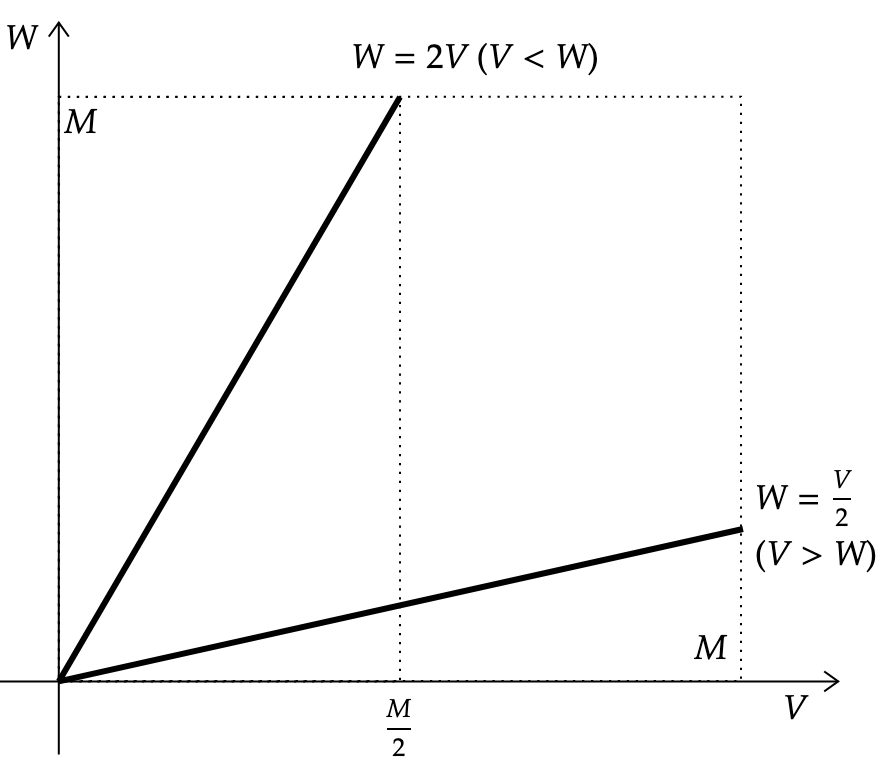
\includegraphics[width=0.9\linewidth]{Images/envelope.png}
\end{center}
\noindent Nous avons suppos\'e que le poids de probabilit\'e sur chaque branche de $\Omega$ est $1/2$; i nous supposons en outre, disons, que la valeur du ch\`eque est aussi possible d'être l'une des valeurs admissibles sur ces branches, alors la loi conjointe est
$$P(V,W)=\begin{cases}
\frac{1}{M} & \text{if $V<W$} \\
\frac{1}{2M} & \text{if $V>W$} \\
0 & \text{otherwise}
\end{cases}$$
et les attentes \'enum\'er\'ees ci-dessus sont
$$E[V\mid V<W]=\int_{V<W}\!\!\!\!\!\!\!\!\!\!\! V\cdot P(V,W)\, d\Omega = \int_{0}^{M/2}\!\!\!\!\!\!\!\!V\cdot\frac{1}{M}\, dV=\frac{M}{8} $$ et $$E[V\mid V>W]=\int_{V>W}\!\!\!\!\!\!\!\!\!\!\! V\cdot P(V,W)\, d\Omega = \int_{0}^{M}\!\!\!\!V\cdot\frac{1}{2M}\, dV=\frac{M}{4}.$$ Par cons\'equent, $$E[W]=\frac{M}{8}+0.25\cdot \frac{M}{4}=\frac{3M}{16}$$ et $$E[V]=0.5\cdot \frac{M}{8}+0.5\cdot \frac{M}{4}=\frac{3M}{16},$$ et le fait de changer d'enveloppe ne change pas la valeur pr\'evue du r\'esultat. Il n'y a pas de paradoxe, pas de cycle infini.
\end{Exemple}

\begin{Exemple} \textbf{ Bayes dans la salle d'audience.} Apr\`es la mort soudaine de ses deux fils, Sally Clark a \'et\'e condamn\'ee par un tribunal britannique \`a la prison \`a vie en 1996. Entre autres erreurs, le t\'emoin expert Sir Roy Meadow avait mal interpr\'et\'e la faible probabilit\'e de la mort subite des deux b\'eb\'es comme une faible probabilit\'e de l'innocence de Clark. Apr\`es une longue campagne, qui comprenait la r\'efutation des statistiques de Meadow en utilisant les statistiques bay\'esiennes, Clark a \'et\'e lib\'er\'ee en 2003. Bien que l'innocence de Clark n'ait pas pu être prouv\'ee hors de tout doute \`a l'aide de telles m\'ethodes, sa culpabilit\'e n'a non plus pu être \'etablie hors de tout doute raisonnable et elle a \'et\'e innocent\'ee. Un article int\'eressant de la situation peut être trouv\'e en ligne \cite{BDA_NNN}.
\end{Exemple}

%----------------------------------------------------------------------------------------
%----------------------------------------------------------------------------------------
\section{Pourquoi utiliser les m\'ethodes bay\'esiennes}
Comme nous l'avons vu pr\'ec\'edemment, les m\'ethodes bay\'esiennes pr\'esentent un certain nombre de caract\'eristiques puissantes: elles permettent aux analystes de
\begin{itemize}[noitemsep]
	\item int\'egrer des connaissances pr\'ealables sp\'ecifiques sur les param\`etres d'int\'erêt;
  \item mettre \`a jour de façon logique les connaissances sur le param\`etre apr\`es avoir observ\'e les donn\'ees relatives \`a l'\'echantillon;
  \item faire des d\'eclarations de probabilit\'e formelles sur les param\`etres d'int\'erêt;
  \item pr\'eciser les hypoth\`eses du mod\`ele et v\'erifier sa qualit\'e et sa sensibilit\'e \`a propos de ces hypoth\`eses de mani\`ere simple;
  \item fournir des lois de probabilit\'e plutôt que des estimations ponctuelles, et 
  \item traiter les valeurs des donn\'ees dans l'\'echantillon comme \'etant interchangeables. 
\end{itemize} 

\subsection{Probl\`emes et solutions}
En particulier, les m\'ethodes bay\'esiennes sont indiqu\'ees afin de r\'esoudre un certain nombre de d\'efis probl\'ematiques dans l'analyse des donn\'ees.
\begin{enumerate}
\item L'ensemble de donn\'ees est petit, mais des informations externes connexes sont disponibles: utiliser les informations dans une a priori. 
\item Le mod\`ele est extrêmement flexible (mod\`ele \`a forte variance) et il est donc sujet \`a un \textbf{overfitting} (sur-ajustement): utilisez des a priori avec des niveaux proches de 0 (ce qui est \`a peu pr\`es \'equivalent au concept de r\'egularisation dans le Machine Learning (l'apprentissage machine).
\item Il est int\'eressant de d\'eterminer la vraisemblance des valeurs des param\`etres, plutôt que de se contenter de produire une " meilleure estimation ": construire la distribution a posteriori complet pour le param\`etre(s) et/ou la variable d'int\'erêt. 
\end{enumerate}
\subsection{Test A/B Bay\'esien}
Le test $A/B$ est un excellent outil pour d\'ecider de mettre en place ou non des caract\'eristiques incr\'ementales. Pour effectuer un test $A/B$, nous divisons les utilisateurs au hasard en un groupe de test et un autre de contrôle, puis fournir la nouvelle caract\'eristique au groupe de test tout en laissant le groupe de contrôle continuer \`a d\'ecouvrir la version actuelle du produit. \par Si la proc\'edure de randomisation est appropri\'ee, nous pourrons peut-être attribuer toute diff\'erence de r\'esultats entre les deux groupes aux changements que nous mettons en place sans avoir \`a tenir compte d'autres sources de variation affectant le comportement des utilisateurs. Avant d'agir sur ces r\'esultats, cependant, il est important de comprendre la vraisemblance que toute diff\'erence observ\'ee soit simplement due au hasard plutôt qu'\`a une modification du produit. \par Par exemple, il est parfaitement possible d'obtenir des rapports $F/P$ diff\'erents entre deux pi\`eces de monnaie \'equitables si nous effectuons seulement une nombre limit\'e des tirages au sort; De la même mani\`ere, il est possible d'observer un changement entre les groupes $A$ et $B$ même si le comportement de l'utilisateur sous-jacent est identique.
\begin{Exemple} (D\'eduit de \cite{BDA_N13}) 
Wakefield Tiles est une entreprise qui vend des carreaux de sol par correspondance. Elle essaie de devenir un acteur dynamique sur le march\'e lucratif de Chelsea en offrant un nouveau type de carreaux aux entrepreneurs de la r\'egion. Le service de marketing a men\'e une \'etude pilote et a essay\'e deux m\'ethodes de marketing diff\'erentes:
\begin{itemize}[noitemsep]
	\item $A$ -- l'envoi par courrier d'une brochure color\'ee pour inviter les entrepreneurs \`a visiter la salle d'exposition de l'entreprise;
	\item $B$ -- l'envoi d'une brochure color\'ee par courrier pour inviter les entrepreneurs \`a visiter la salle d'exposition de l'entreprise, tout en incluant des \'echantillons de carreaux gratuits.
\end{itemize}
Le service marketing a envoy\'e $16$ colis postaux de type $A$ et $16$ colis postaux de type $B$. Quatre Chelseaites qui ont reçu un colis de type $A$ ont visit\'e la salle d'exposition, tandis que $8$ de ceux qui ont reçu un colis de type $B$ ont fait de même. L'entreprise est consciente que:
\begin{itemize}[noitemsep]
\item l'exp\'edition de type $A$ coûte 30 \$ (comprend les frais d'impression et les frais de port);
\item l'exp\'edition de type $B$ coûte 300\$ (comprend en plus le coût des \'echantillons de tuiles gratuits);
\item une visite \`a la salle d'exposition rapporte, en moyenne, 1000\$ de revenus au cours de l'ann\'ee suivante.
\end{itemize}
Laquelle des m\'ethodes (A ou B) est la plus avantageuse pour Wakefield Tile? \newl
\textbf{Solution:} la solution bay\'esienne exige la construction d'une loi a priori et \textbf{d'un mod\`ele g\'en\'eratif}; dans le cadre du mod\`ele g\'en\'eratif, nous devrons produire $n$ r\'epliques d'\'echantillons \`a partir de la loi binomiale (qui peut être fait dans R en utilisant \texttt{rbinom(n,size,prob)}). \par La loi binomiale simule \texttt{n} fois le nombre de "succ\`es" lors des essais de \texttt{taille} (envois postaux), où la probabilit\'e de "succ\`es" est \texttt{prob}.  Une a priori couramment utilis\'e pour \texttt{prob} est la loi uniforme $U(0,1)$, \`a partir de laquelle nous pouvons \'echantillonner dans R \textit{via} \texttt{runif(1, min = 0, max = 1)}.  
\begin{lstlisting}
# Le nombre de r\'ep\'etition de la distribution a priori
n.draws <- 200000

# la distribution a priori
# Ce g\'en\`ere la probabilit\'e des
# succ\`es des exp\'editions A et B, 
# pour toutes les r\'ep\'etitions
prior <- data.frame(p.A = runif(n.draws, 0, 1), p.B = runif(n.draws, 0, 1))

# Le mod\`ele g\'en\'eratif
# Cela nous indique le nombre de # visiteurs \`a attendre
# pour les exp\'editions des types # A et B 
generative.model <- function(p.A, p.B) {
  visitors.A <- rbinom(1, 16, p.A)
  visitors.B <- rbinom(1, 16, p.B)
  c(visitors.A = visitors.A, visitors.B = visitors.B)
}

# simuler les donn\'ees des 
# param\`etres \`a partir de l'a 
# priori et du mod\`ele g\'en\'eratif 
# Cela va simuler le vrai nombre 
# des visiteurs pour chaque 
# r\'ep\'etition
sim.data <- as.data.frame(t(sapply(1:n.draws, function(i) {
  generative.model(prior$p.A[i], prior$p.B[i])})))

# On garde seulement les 
# probabilit\'es a priori pour 
# lequelles le mod\`ele g\'en\'eratif
# correspond aux donn\'ees observ\'ees 

posterior <- prior[sim.data$visitors.A == 4 & sim.data$visitors.B == 8, ] 

# Visualiser les a posteriori
par(mfrow = c(1,3))
hist(posterior$p.A, main = "la distribution a posteriori -- la probabilit\'e de succ\`es pour l'exp\'edition de type A", xlab="p.A") 
hist(posterior$p.B, main = "L'a posteriori -- la probabilit\'e de succ\`es pour l'exp\'edition de type B", xlab="p.B")
plot(posterior,main = "Nuage de points de la probabilit\'e de succ\`es pour les exp\'editions de types A et B", xlab="p.A", ylab="p.B")
\end{lstlisting}

Les lois a posteriori de la probabilit\'e de succ\`es pour chaque type d'exp\'edition est illustr\'e dans la figure ci- dessous.
\begin{center}
  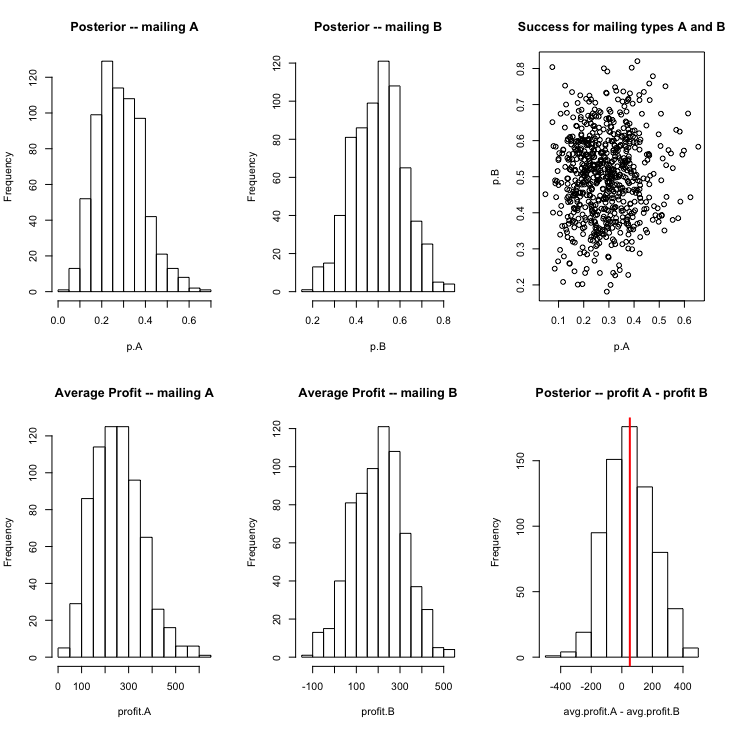
\includegraphics[width=\linewidth]{Images/example12e.png}
\end{center}
Afin d'estimer le b\'en\'efice moyen pour chaque type d'envoi, nous utilisons les lois a posteriori pour la probabilit\'e de succ\`es.   
\begin{lstlisting}
# Calculer le moyen estim\'e du   profit pour chaque type d'envoi
avg.profit.A <- -30 + posterior$p.A * 1000 
avg.profit.B <- -300 + posterior$p.B * 1000 
hist(avg.profit.A, main = "Average Profit -- mailing A", xlab="profit.A") 
hist(avg.profit.B, main = "Average Profit -- mailing B", xlab="profit.B")
\end{lstlisting}
\noindent Le b\'en\'efice pr\'evu est donc donn\'e par le code suivant:
\begin{lstlisting}
#Le profit estim\'e total
hist(avg.profit.A - avg.profit.B)
expected.avg.profit.diff <- mean(avg.profit.A - avg.profit.B)
abline(v = expected.avg.profit.diff , col = "red", lwd =2)
\end{lstlisting}
Le profit pr\'evu pour un envoi de type $A$ est d'environ 52\$ plus \'elev\'e que pour un envoi de type $B$ (vos chiffres peuvent varier). Dans ce contexte, il semble pr\'ef\'erable de garder les choses simples.
\end{Exemple}


%----------------------------------------------------------------------------------------
% Summary
%----------------------------------------------------------------------------------------
\newpage
\section{Bilan}
\begin{description}
	\item \textbf{Quoi?}
	   \begin{itemize}
		   \item L'analyse bay\'esienne des donn\'ees est une m\'ethode flexible qui s'adapte \`a tout type de mod\`ele statistique. 
			 \item Le maximum de vraisemblance est en fait un cas particulier de l'ajustement du mod\`ele bay\'esien.
	   \end{itemize}
	\item \textbf{Pourquoi?}
			\begin{itemize}
				\item Permet de d\'efinir des mod\`eles fortement configurables.
				\item Permet d'inclure des informations provenant de nombreuses sources, comme les donn\'ees et les connaissances d'experts.
				\item Quantifie et conserve l'incertitude des estimations et des pr\'evisions des param\`etres.
			\end{itemize}
	\item \textbf{Comment?}
	\begin{itemize}
	       \item R! En utilisant ABC, MCMCpack, JAGS, STAN, R-inla, Python, etc.
	       \end{itemize}
\end{description}

%---------------------------------------------------------------------------------------
% ---------- Appendix A-----------------------------------------------------------------
%---------------------------------------------------------------------------------------
\appendix

%---------------------------------------------------------------------------------------
% ---------- Appendix B-----------------------------------------------------------------
%---------------------------------------------------------------------------------------
\section*{Exercices -- Solutions}
\begin{itemize}
	
\item \textbf{Exercice }\ref{ex1.4.1}:  
$$ P(L\mid Y) = \frac{P(Y\mid L) P(L)}{P(Y)}$$
Notez que $$P(Y) = P(Y,L) + P(Y,\overline{L}) = P(Y\mid L) P(L) + P(Y\mid \overline{L}) P(\overline{L}),$$ Donc
$$P(L\mid Y) =\frac{(.55)(.52)}{(.55)(.52)+(.85)(.48)} = 0.41.$$

\item \textbf{Exercice }\ref{ex1.4.2}: 
\begin{description}
\item[\'etape 1:] affecter des \'ev\'enements \`a $A$ ou $X$. Vous voulez savoir quelle est la probabilit\'e qu'une femme ait un cancer, compte tenu d'une mammographie positive. Pour ce probl\`eme, le fait d'avoir un cancer est $A$ et un r\'esultat positif est $X$.
\item[\'etape 2:] faites une liste des \'el\'ements de l'\'equation (cela facilite le travail sur l'\'equation effective):
$$P(A) = 0.01, P(\overline{A})= 0.99, P(X\mid A)=0.9, P(X\mid \overline{A}).$$ 
\item[\'etape 3:] ins\'erer les \'el\'ements dans l'\'equation et r\'esoudre. Notez que comme il s'agit d'un test m\'edical, nous avons
$$\frac{0.9\cdot 0.01}{(0.9)(0.01)+(0.08)(0.99)} = 0.10.$$ 
La probabilit\'e qu'une femme ait un cancer, en cas de r\'esultat positif au test, est donc de 10\%. 
\end{description}

\newpage\noindent\item \textbf{Exercice }\ref{ex3.5.1}
\begin{enumerate}
	\item justifier un a priori,on pourrait dire que notre force d'\'equit\'e est \'equivalant \`a avoir d\'ej\`a vu la pi\`ece de monnaie être retourn\'ee 100 fois et avoir obtenu un $F$ dans 50\% de ces lancements. Par cons\'equent, la distribution a priori serait  $\text{Beta}(\theta\mid 50,50)$ (ce n'est pas la seule bonne r\'eponse, bien sûr; vous pourriez plutôt être plus confiants et utiliser, disons,  $\text{Beta}(\theta\mid 500,500)$ si vous supposez que vous avez d\'ej\`a vu $1,000$ lancement avec 50\% de faces).\\
	L'a posteriori est alors  $\text{Beta}(\theta\mid 50+9,50+1)$, qui a une moyenne de $\frac{59}{59+51} = 0.536$. C'est la probabilit\'e pr\'edite de faces pour le prochain (11th) lancement.
\item Dans ce cas, nous utilisons une loi $\text{Beta}(\theta\mid 0.5,0.5)$ a priori, comme celui utilis\'e dans Exemple \ref{Ex:unusualprior}, car il exprime une croyance que la pi\`ece est soit \`a biais de face, soit \`a biais de piles car il exprime une croyance que la pi\`ece est soit \`a biais de face, soit \`a biais de piles. \newl L'a posteriori est donc $\text{Beta}(\theta\mid 0.5+9,0.5+1)$, qui a une moyenne de $\frac{9.5}{9.5+1.5} = 0.863$. C'est la probabilit\'e pr\'edite de faces pour le prochain (11\`eme) lancement. Notez qu'elle est tout a fait diff\'erente de la conclusion de la Partie 1.
\end{enumerate}


\item \textbf{Solution de l'exercice }\ref{ex4.2.1} \\
Les commandes 
\begin{quote}
\small \texttt{> post = BernBeta(c(1,1),  \\ 
\ \ \ \ \ \ \ \  c(rep(1,40),rep(0,10)))}\\
\texttt{> post = BernBeta(c(1,1),    \\
\ \ \ \ \ \ \ \   c(rep(1,15),rep(0,35)))} \normalsize
\end{quote}
donne le graphe ci-dessous.
\begin{center}
		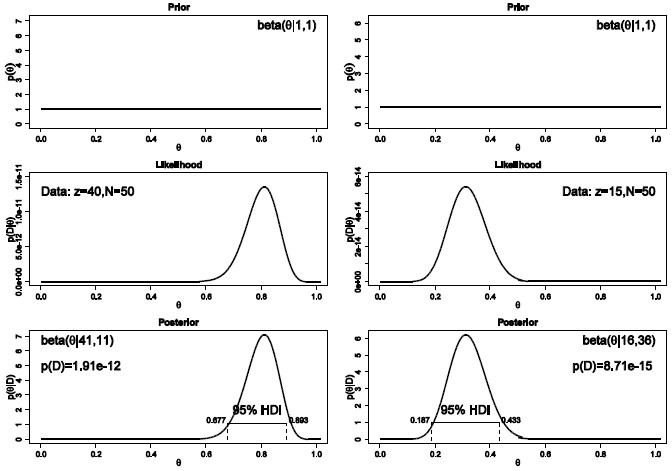
\includegraphics[width=\linewidth]{Images/exsection4.png}
\end{center}
Dans les deux cas, l'intervale HPD de 95\% exclut $\theta=0.5$, et nous concluons donc que les gens sont en effet biais\'es dans leurs r\'eponses, vers F dans le premier cas et vers J dans le second cas. 
\end{itemize}
